% This is the template for the writing report
% Figures and this .tex file should be put in the same folder
% You only need to make changes of this .tex file and submit .pdf after converting this to .pdf
% Ignore other files in this folder
\documentclass{article}
\usepackage{float}
\usepackage{graphicx}
\usepackage{caption}
\usepackage{subcaption}
\usepackage{array}
\usepackage{geometry}
\usepackage{amsmath, bm}
\title{Machine Learning-Based Cryptocurrency Price Prediction} % come up with a good title
\author{Andrew Cooke, Yu Wang, Xinming Dai}
\geometry{left=3cm} 

\begin{document}
\maketitle

\section{Abstract}
\section{Introduction}
	
\section{Data Collection and Description}
\subsection{Tweets from Elon Musk}

The goal was to collect Elon Musk’s tweets and identify which of them were cryptocurrency-related text. Tweepy library in Python was used to access Twitter API, and only the 3200 most recent tweets are available for each user.\\

\noindent A bag of crypto words containing cryptocurrency’s names and symbols was created, and then pre-selected words were used to match crypto-related tweets. 3559 Elon Musk’s tweets from 2021-05-28 to 2022-05-01 were collected, 2.39\% of which consisted of cryptocurrency-related words. He tweeted about crypto up to 5 times a day, but most of the time he didn’t tweet about crypto. Figure 1 indicates that there is a high correlation between whether Elon tweets cryptos and high volatility of Ethereum prices. The highly volatile adjusted closing price returns is related to when Elon tweets about cryptos and the number of his crypto tweets. Returns of less than 5\% are omitted from Figure \ref{fig: tweets_and_returns} because 5\% is within its normal range of volatility.

\begin{figure}[H]
	\centering
	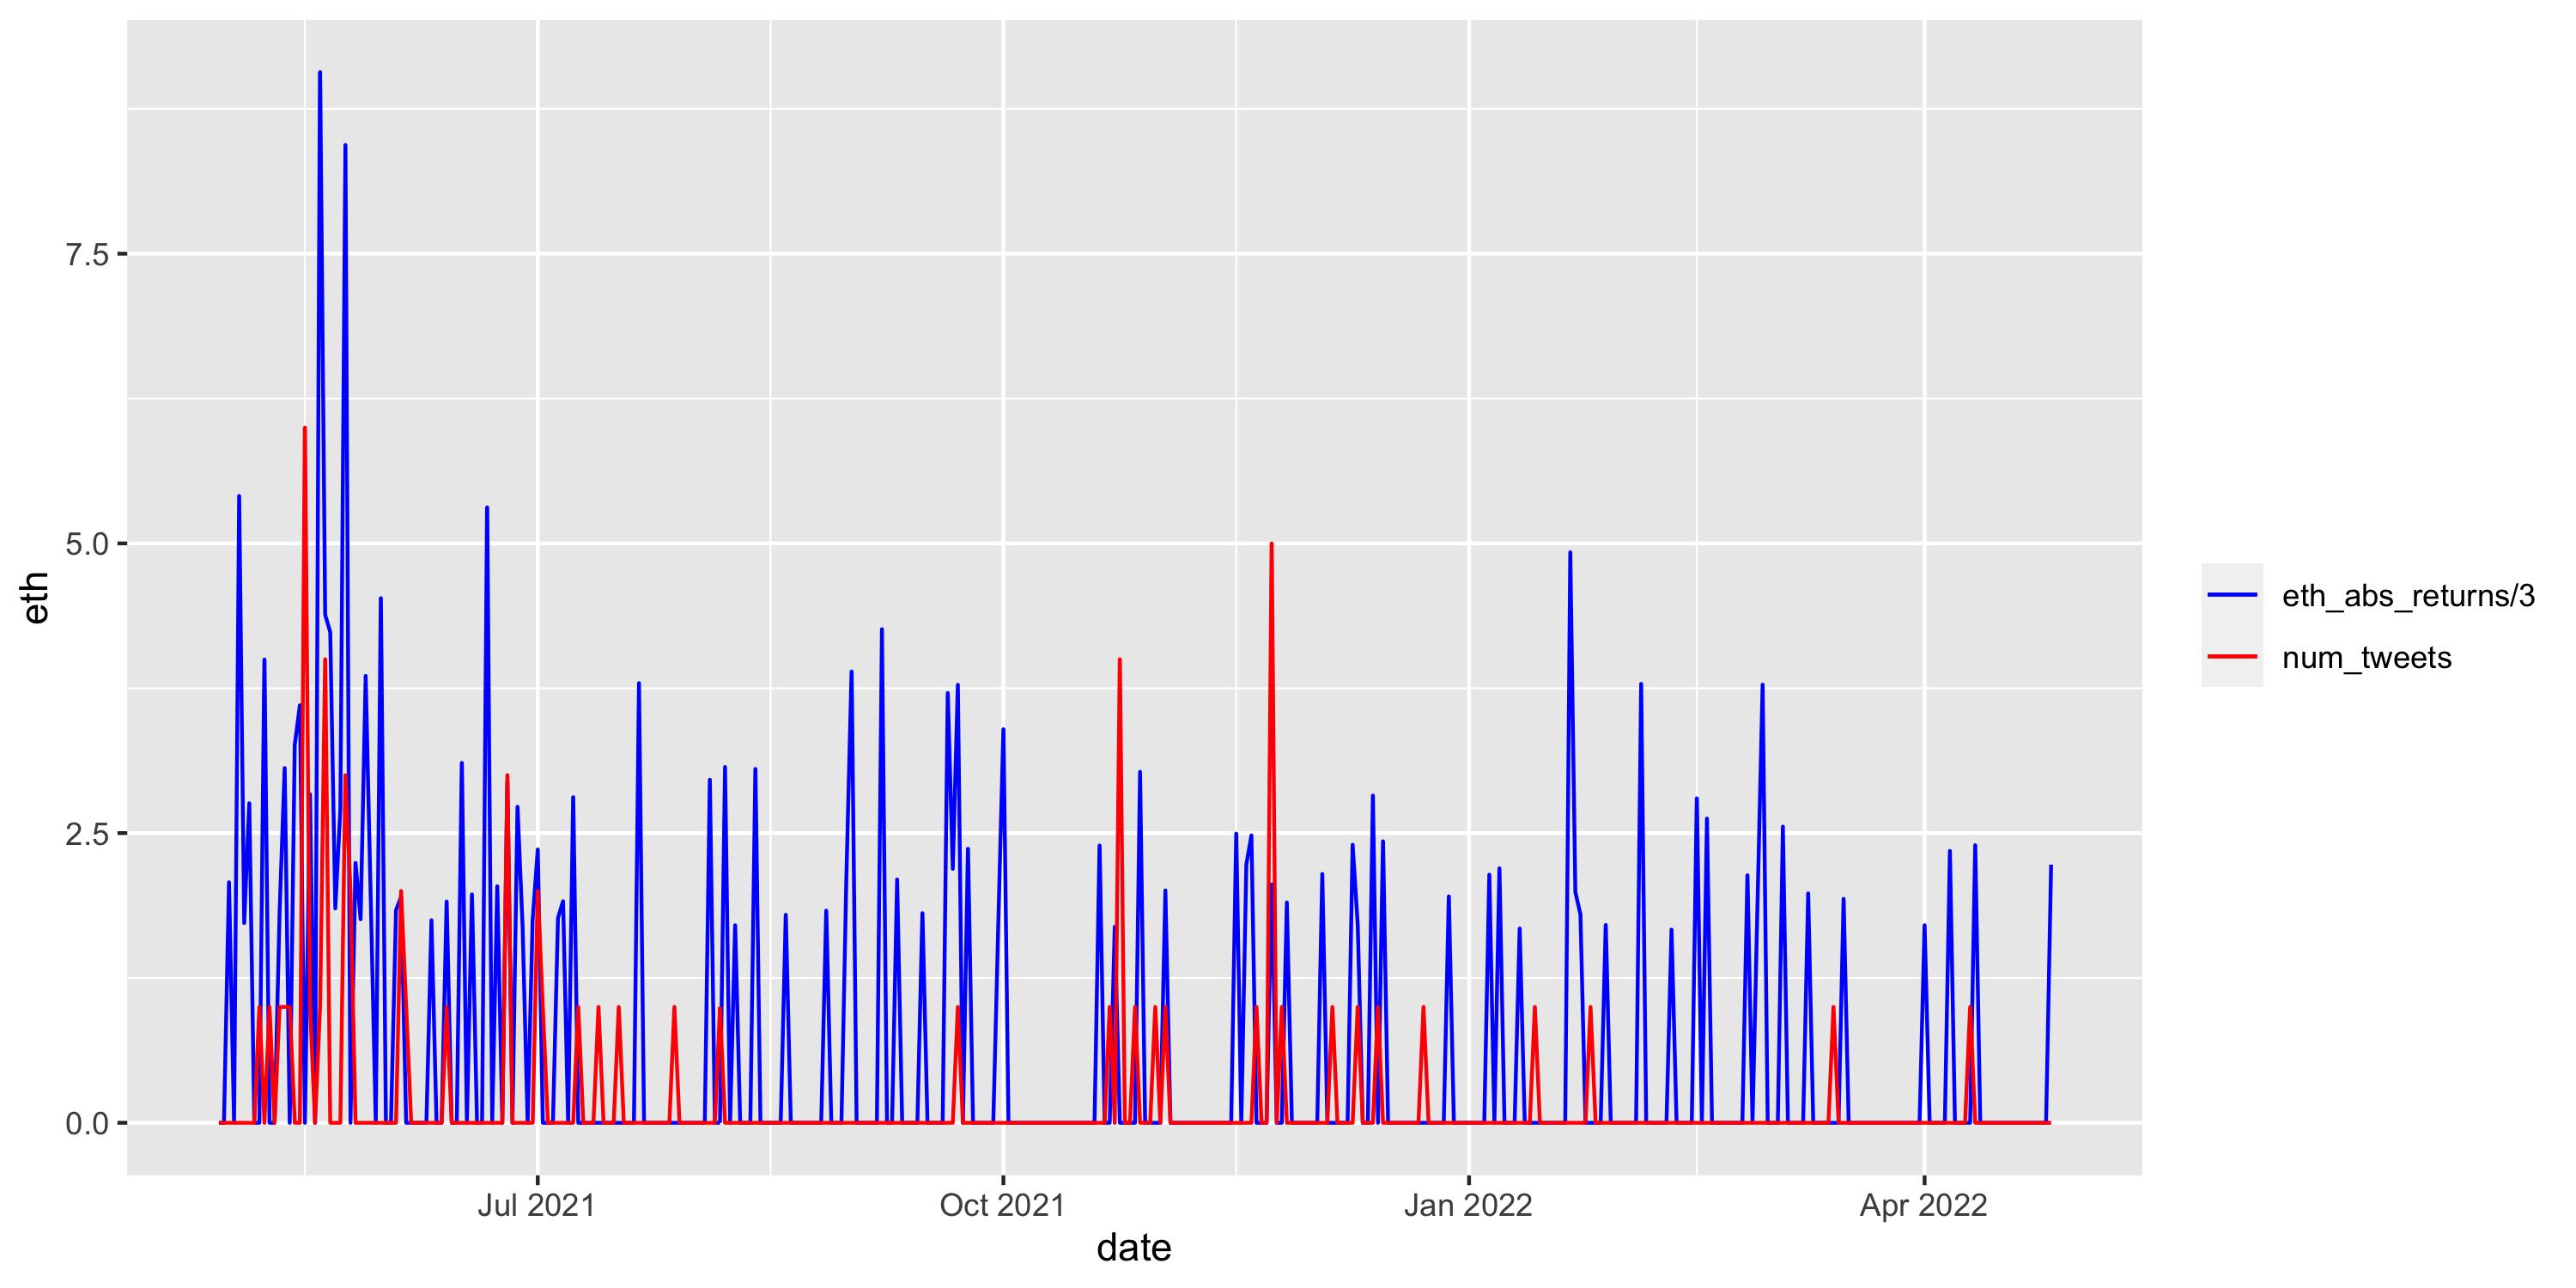
\includegraphics[width=18cm]{../figures/tweets_and_returns.png}
	\caption{The number of tweets and volatility of Ethereum. Ethereum volatility index in this figure was defined as its absolute return divided by 3. }
	\label{fig: tweets_and_returns}
\end{figure}

\subsection{Cryptocurrency Price on Yahoo Fiance}
Another major data source that we use in this project is the cryptocurrency price from Yahoo Finance. All major crypto prices for each day can be easily obtained in R by using the code under the ‘tidyquant’ package, such as tq\_get(), and we made some manipulations on the dataset based on our statistical and modeling needs. For instance, since the predictors and outcome variables in this project are daily returns, calculate by $$\frac{(\text{new adjusted closing price} - \text{old adjusted closing price})}{\text{old adjusted closing price} }*100,$$ we build our own function to help us do this. We also include some descriptions for the Cleaning/compilation/ manipulation process in R via comments. The raw dataset for the crypto prices will look something like the table \ref{Crypto prices} below.

\begin{table}[ht]
\centering
\begin{tabular}{rllllllll}
  \hline
 & symbol & date & open & high & low & close & volume & adjusted \\ 
  \hline
1 & ETH-USD & 2022-04-21 & 3077.83 & 3173.45 & 2962.41 & 2987.48 & 20783591093.00 & 2987.48 \\ 
  2 & ETH-USD & 2022-04-22 & 2986.94 & 3024.85 & 2942.36 & 2964.84 & 16782795477.00 & 2964.84 \\ 
  3 & ETH-USD & 2022-04-23 & 2964.80 & 2975.32 & 2926.74 & 2938.11 & 9116955609.00 & 2938.11 \\ 
  4 & ETH-USD & 2022-04-24 & 2937.35 & 2961.88 & 2922.13 & 2922.73 & 9696829579.00 & 2922.73 \\ 
  5 & ETH-USD & 2022-04-25 & 2922.99 & 3018.42 & 2804.51 & 3009.39 & 22332690614.00 & 3009.39 \\ 
  6 & ETH-USD & 2022-04-26 & 3008.95 & 3026.42 & 2786.25 & 2808.30 & 19052045399.00 & 2808.30 \\ 
   \hline
\end{tabular}
\caption{Crypto prices} 
\label{Crypto prices}
\end{table}

\section{Modeling and Analysis}
In many financial and business fields, the rationale of time series usually plays a critical role in terms of analyzing and predicting cryptocurrency data, such as stock returns. The reason is that the stock price data are taken sequentially in time, and each day’s stock price is highly correlated with the prices on other days. Meanwhile, it also have a correlation with other cryptocurrency prices. Hence, we can’t assume the error are independent. In addition, we usually do not consider its outcome as binary. Based on this idea, we divided our statistical models into two parts. The first part is using simple generalized linear model, such as logistic regression, whereas the second part is using more complex time series models, such as ARIMA, Bayesian structural time series (BSTS), and random forest.\\

\subsection{Model 1: Simple Logistic Regression Model}
A logistic regression model is a very common statistical model to predict a binary outcome, such as True/False, and Yes/No. It simply takes all the input values and outputs the probability of the outcome being True. The mathematics behind the logistical regression model can be interpreted as
$$P(Y_i=1)=logit^{-1}(X_i\bm{\beta})=\frac{e^{X_i\bm{\beta}}}{1+e^{X_i\bm{\beta}}},$$

\noindent where $X_i\bm{\beta}$ refers to the linear predictors.



\begin{itemize}
  	\item XXX
	\item XXX
\end{itemize}


%\begin{figure}[H]
	%\centering
	%\includegraphics[width=12cm]{trips.png}
	%\label{fig:1}
%\end{figure}

\end{document}